\subsection{Track-based Missing Energy}
\label{sec:TkMET}

The vector sum of the transverse momenta (MET) of all particles produced in the primary collision is a key input for BSM triggers at Level-1. For the track-based algorithm described in this section, one of the main challenges is excluding tracks from bad combinations, ``fake tracks," that give high transverse momentum. Though these tracks are rare in pileup after requiring a tight window around the primary vertex z position, events containing these tracks would dominate an L1 MET trigger. The algorithm makes use of track purity requirements in addition to the $\Delta z\left(PV_{z}, trk_{z}\right)$ requirement to reduce the number of events with poorly measured momentum balance.

The track purity selection is based mainly on the confines of the detector, the track reconstruction algorithm, and the available track fit quality parameters. The track $p_{T}$ and $\eta$ requirements shown in Table~\ref{tab:trkpurity} are based on the minimal $p_{T}$ of tracks that can be reconstructed reliably and the tracking acceptance. The minimal number of track layers is also based on the minimal requirement for the track fit. There is a further requirement that 4 of the track layers must also have stubs to remove any 4-stub tracks that were created with only hits in 3 layers. Requirements on the track fit quality measured as $\chi^{2}_{n.dof}$ is set to a minimum of 50 to reduce tracks that are poorly reconstructed. To further reject fake tracks, a new variable, bend consistency, $\chi^{2}_{bend}$ is measured. This measure of the bend of the track is uncorrelated to the $\chi^{2}_{n.dof}$ from the track fit. $\chi^{2}_{bend}$ is calculated based on the horizontal distance between the two consecutive track hits in a track module, the stubs. The bend consistency quantifies how compatible the bend of the track hits measured in the detector is with the reconstructed track $p_{T}$. The bend consistency variable is defined as:
\begin{equation}
\chi^{2}_{bend} =~ \frac{1}{N_{stubs}} \sum_{i=1}^{N_{stubs}}\Big(\frac{\beta_i - \beta_i^{exp}}{\sigma_{i}}\Big)^2
\end{equation}
where $N_{stubs}$ is the total number of stubs comprising the track, $\beta_{i}$ is the measured bend angle for stub i, and $\beta_i^{exp}$ is the expected bend angle based on the track. A bad combination of track hits tends to have a large value of bend consistency compared to well-reconstructed tracks. The cut on $\chi^{2}_{bend}$ is optimized to lower the fraction of poorly reconstructed tracks that are included in the MET calculation, as well as maintain a reasonable L1 data-taking rate for a track-based MET trigger.



\begin{table}[h]
\begin{tabular}{|c|c|}
Track Variable & Cut\\
$N_{stubs}$ per track layer&$\geq 4$ \\
$p_{T}$ & 2~GeV \\
$\chi^{2}_{n.dof}$ & 50 \\
$\chi^{2}_{bend}$  & 1.75 \\

\end{tabular}
\caption{ L1 track purity requirements for tracks input to both the MET computation and the L1 track-based jet clustering. Cuts are optimized to preserve a sharp turn-on in track-based MET, $H_{T}$, and $H^{miss}_{T}$ rejecting the bulk of ``fake" tracks from bad combinations of track hits.}
\label{tab:trkpurity}
\end{table}

The L1 vertex described in the TSA firmware algorithm in Section~\ref{sec:FastHisto} is input to the L1 track-based MET algorithm. A window of $\Delta z\left(PV_{z}, trk_{z}\right)$ is required for pseudo-rapidity regions within the tracking acceptance. Table~\ref{tab:zwindows} shows the range of values for the allowed range of track-z around the measured primary vertex z. Central tracks allow for a tight window of 0.4 cm while more forward tracks need a wider z-window (as large as 2.2 cm) to include tracks within $3\sigma$ of the Gaussian track z-resolution.
\begin{table}[h]
\begin{tabular}{|c|c|}
$\eta$ range & $\vert \Delta z\left(PV_{z}, trk_{z}\right) \vert$  [cm] \\
 $0\leq \eta < 0.7$ & 0.4\\
$0.7\leq \eta <1.0 $& 0.6\\
$1.0\leq \eta < 1.2 $ & 0.76\\
$1.2\leq \eta < 1.6$ & 1.0 \\
$1.6\leq \eta <  2.0 $& 1.7 \\
$2.0\leq  \eta < 2.4 $ & 2.2 \\
\end{tabular}
\caption{Minimum $\Delta z $ requirements between the primary vertex and track $z_{0}$ in each pseudo-rapidity region for track selection for the MET algorithm. }
\label{tab:zwindows}
\end{table}

To gauge the performance of track-based MET, we compare the reconstructed track-based MET to simulated tracking particles, which are the simulation-level trajectories of charged particles in an event. The tracking particles are used to compute the simulated MET using the same algorithm as the reconstructed L1 tracks. This gives the expected L1 track MET in the case where no fake tracks are included in the MET computation. Figure~\ref{fig:TkMETPerformance} shows the data-taking L1 rate for the track MET from the reconstructed tracks and the tracking particles. Applying only the $\vert \Delta z\left(PV_{z}, trk_{z}\right) \vert$ cut in Table~\ref{tab:zwindows} gives an L1 rate of 35 kHz for a track-based MET threshold at 200 GeV. Applying the full track selection in Table~\ref{tab:trkpurity} shows that this threshold is lowered to 60 GeV, which is the same threshold as when only simulated charged particle trajectories are used for the MET computation.
This allows a low trigger turn-on for offline-MET for BSM models like the BSM Stop signal. The trigger turn-on at 95$\%$ is lowered from 500 GeV applying only the primary vertex constraint to 300 Gev when including the full selection of tracks.
%The trigger turn-on in the BSM stop sample gives 95$\%$ efficiency at 350~GeV for generator-level MET.
%%%%Include preliminary plots from Emily%%%%%%%%%%%
\begin{figure}
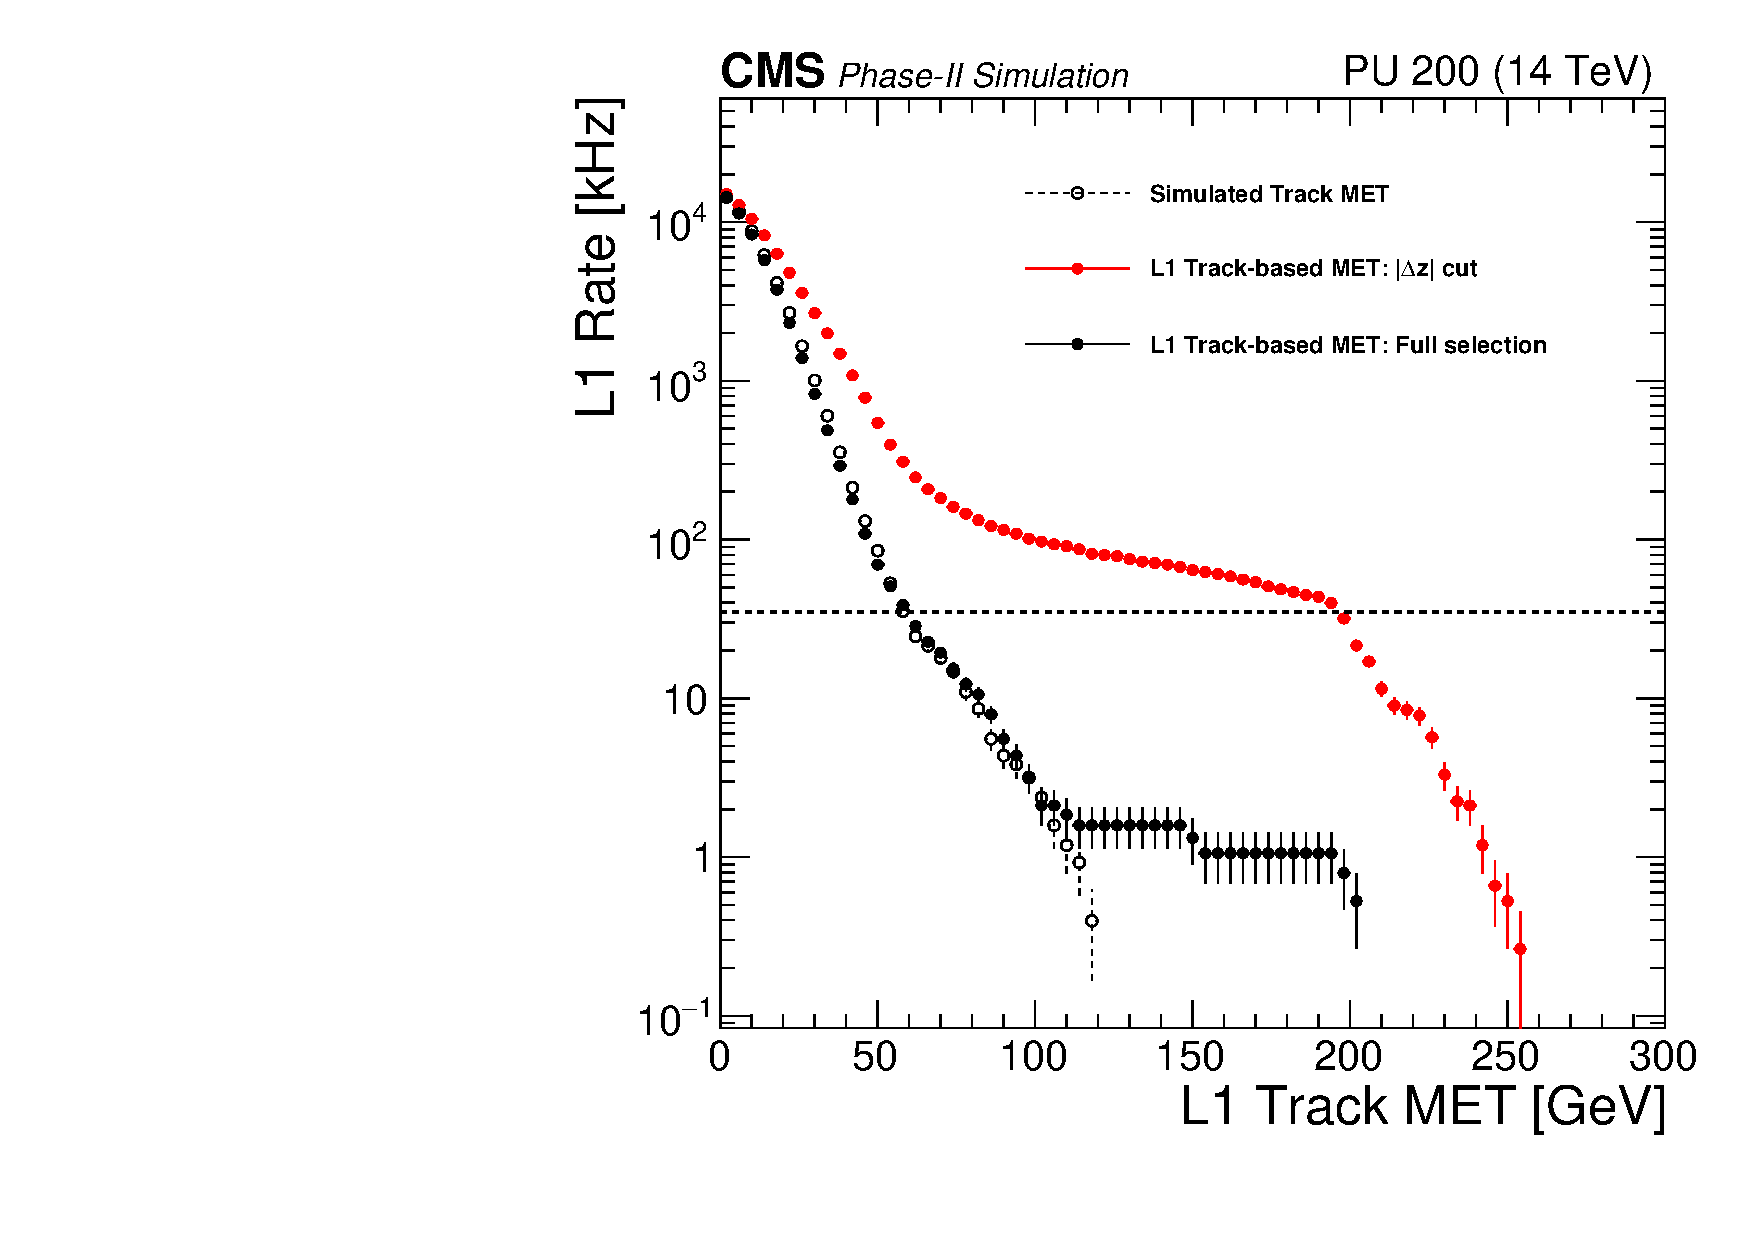
\includegraphics[width=0.45\textwidth ]{MinBiasTKMETRatePlot.pdf}
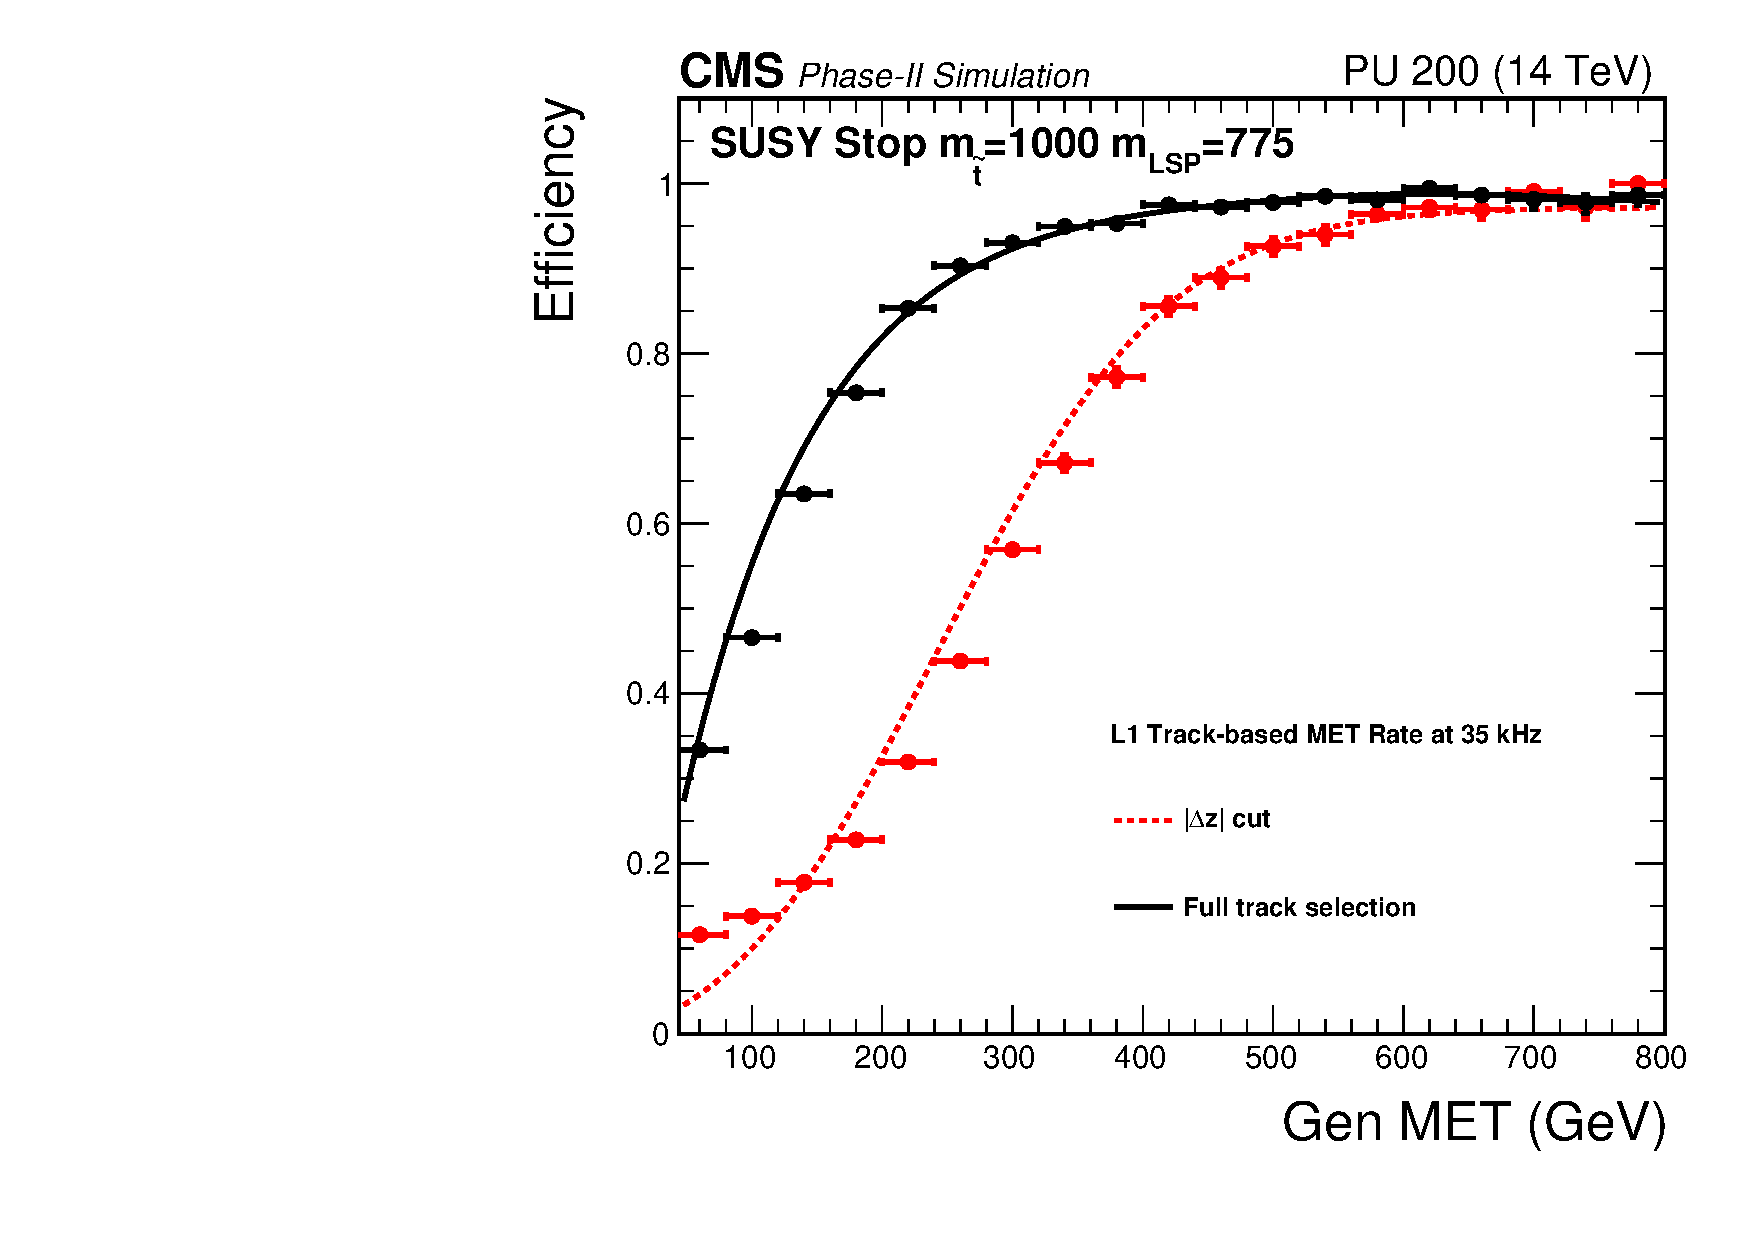
\includegraphics[width=0.45\textwidth ]{turnonMET.pdf}
\caption{The track MET threshold for a minimum bias sample. The full track selection reduces the threshold from 200 GeV to 60 GeV, which is closely aligned with the threshold from the simulated tracks.}
\label{fig:TkMETPerformance}
\end{figure}


\begin{figure}
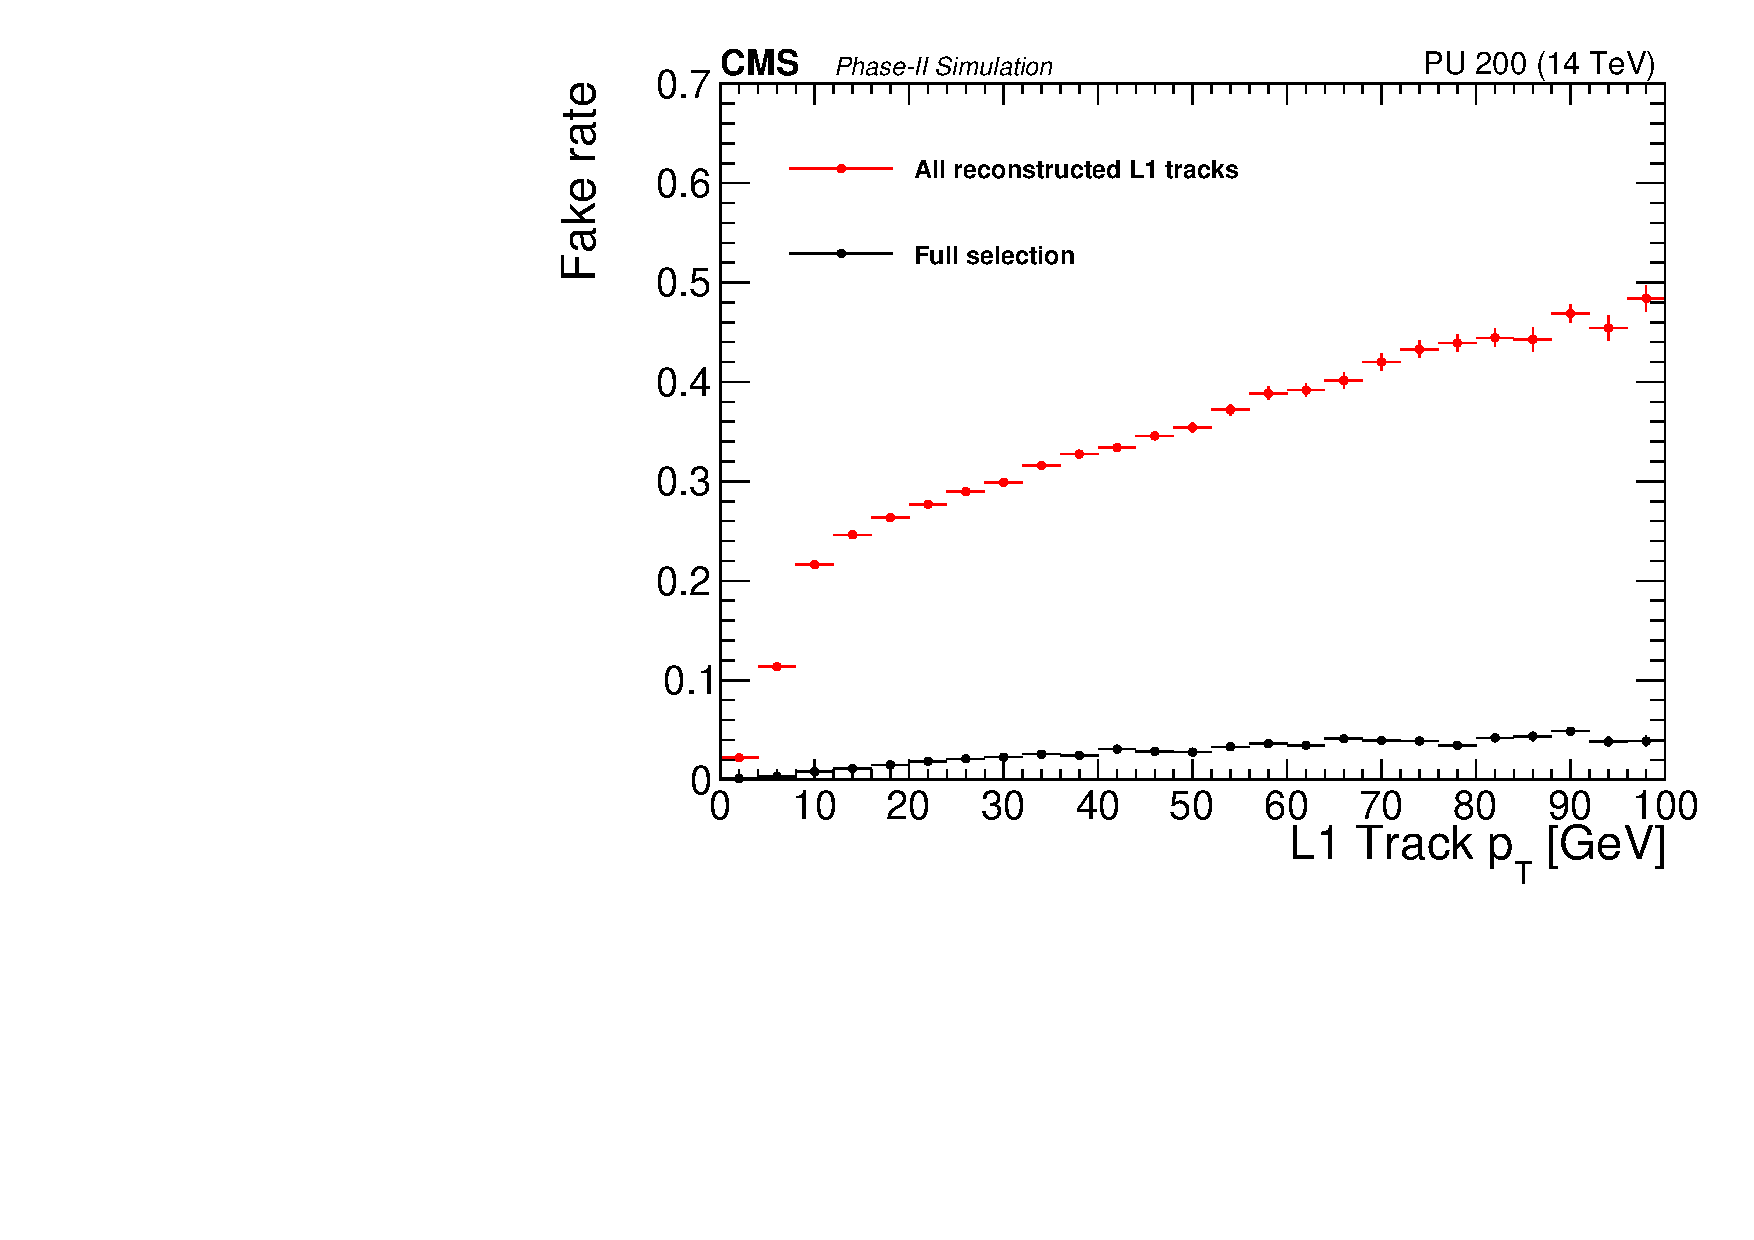
\includegraphics[width=0.45\textwidth ]{StopSamplePUFakeRatePt.pdf}
\caption{The full track selection greatly reduces the fake rate, the percentage of bad-combination tracks that cannot be matched to truth-information to all reconstructed tracks. The reduction of the fake rate is an important part as the fake tracks contribute erroneous momentum, which can cause these events to dominate an L1 MET trigger.}
\label{fig:TkFakeRate}
\end{figure}

%Including these criteria for the optimized track MET measurement reduces the threshold at a data-taking rate of 35 kHz from 200 GeV to 60 GeV. This threshold corresponds closely to the simulated true track MET performance.
